% Options for packages loaded elsewhere
\PassOptionsToPackage{unicode}{hyperref}
\PassOptionsToPackage{hyphens}{url}
\PassOptionsToPackage{dvipsnames,svgnames,x11names}{xcolor}
%
\documentclass[
  letterpaper,
  DIV=11,
  numbers=noendperiod]{scrartcl}

\usepackage{amsmath,amssymb}
\usepackage{lmodern}
\usepackage{iftex}
\ifPDFTeX
  \usepackage[T1]{fontenc}
  \usepackage[utf8]{inputenc}
  \usepackage{textcomp} % provide euro and other symbols
\else % if luatex or xetex
  \usepackage{unicode-math}
  \defaultfontfeatures{Scale=MatchLowercase}
  \defaultfontfeatures[\rmfamily]{Ligatures=TeX,Scale=1}
\fi
% Use upquote if available, for straight quotes in verbatim environments
\IfFileExists{upquote.sty}{\usepackage{upquote}}{}
\IfFileExists{microtype.sty}{% use microtype if available
  \usepackage[]{microtype}
  \UseMicrotypeSet[protrusion]{basicmath} % disable protrusion for tt fonts
}{}
\makeatletter
\@ifundefined{KOMAClassName}{% if non-KOMA class
  \IfFileExists{parskip.sty}{%
    \usepackage{parskip}
  }{% else
    \setlength{\parindent}{0pt}
    \setlength{\parskip}{6pt plus 2pt minus 1pt}}
}{% if KOMA class
  \KOMAoptions{parskip=half}}
\makeatother
\usepackage{xcolor}
\setlength{\emergencystretch}{3em} % prevent overfull lines
\setcounter{secnumdepth}{5}
% Make \paragraph and \subparagraph free-standing
\ifx\paragraph\undefined\else
  \let\oldparagraph\paragraph
  \renewcommand{\paragraph}[1]{\oldparagraph{#1}\mbox{}}
\fi
\ifx\subparagraph\undefined\else
  \let\oldsubparagraph\subparagraph
  \renewcommand{\subparagraph}[1]{\oldsubparagraph{#1}\mbox{}}
\fi

\usepackage{color}
\usepackage{fancyvrb}
\newcommand{\VerbBar}{|}
\newcommand{\VERB}{\Verb[commandchars=\\\{\}]}
\DefineVerbatimEnvironment{Highlighting}{Verbatim}{commandchars=\\\{\}}
% Add ',fontsize=\small' for more characters per line
\usepackage{framed}
\definecolor{shadecolor}{RGB}{241,243,245}
\newenvironment{Shaded}{\begin{snugshade}}{\end{snugshade}}
\newcommand{\AlertTok}[1]{\textcolor[rgb]{0.68,0.00,0.00}{#1}}
\newcommand{\AnnotationTok}[1]{\textcolor[rgb]{0.37,0.37,0.37}{#1}}
\newcommand{\AttributeTok}[1]{\textcolor[rgb]{0.40,0.45,0.13}{#1}}
\newcommand{\BaseNTok}[1]{\textcolor[rgb]{0.68,0.00,0.00}{#1}}
\newcommand{\BuiltInTok}[1]{\textcolor[rgb]{0.00,0.23,0.31}{#1}}
\newcommand{\CharTok}[1]{\textcolor[rgb]{0.13,0.47,0.30}{#1}}
\newcommand{\CommentTok}[1]{\textcolor[rgb]{0.37,0.37,0.37}{#1}}
\newcommand{\CommentVarTok}[1]{\textcolor[rgb]{0.37,0.37,0.37}{\textit{#1}}}
\newcommand{\ConstantTok}[1]{\textcolor[rgb]{0.56,0.35,0.01}{#1}}
\newcommand{\ControlFlowTok}[1]{\textcolor[rgb]{0.00,0.23,0.31}{#1}}
\newcommand{\DataTypeTok}[1]{\textcolor[rgb]{0.68,0.00,0.00}{#1}}
\newcommand{\DecValTok}[1]{\textcolor[rgb]{0.68,0.00,0.00}{#1}}
\newcommand{\DocumentationTok}[1]{\textcolor[rgb]{0.37,0.37,0.37}{\textit{#1}}}
\newcommand{\ErrorTok}[1]{\textcolor[rgb]{0.68,0.00,0.00}{#1}}
\newcommand{\ExtensionTok}[1]{\textcolor[rgb]{0.00,0.23,0.31}{#1}}
\newcommand{\FloatTok}[1]{\textcolor[rgb]{0.68,0.00,0.00}{#1}}
\newcommand{\FunctionTok}[1]{\textcolor[rgb]{0.28,0.35,0.67}{#1}}
\newcommand{\ImportTok}[1]{\textcolor[rgb]{0.00,0.46,0.62}{#1}}
\newcommand{\InformationTok}[1]{\textcolor[rgb]{0.37,0.37,0.37}{#1}}
\newcommand{\KeywordTok}[1]{\textcolor[rgb]{0.00,0.23,0.31}{#1}}
\newcommand{\NormalTok}[1]{\textcolor[rgb]{0.00,0.23,0.31}{#1}}
\newcommand{\OperatorTok}[1]{\textcolor[rgb]{0.37,0.37,0.37}{#1}}
\newcommand{\OtherTok}[1]{\textcolor[rgb]{0.00,0.23,0.31}{#1}}
\newcommand{\PreprocessorTok}[1]{\textcolor[rgb]{0.68,0.00,0.00}{#1}}
\newcommand{\RegionMarkerTok}[1]{\textcolor[rgb]{0.00,0.23,0.31}{#1}}
\newcommand{\SpecialCharTok}[1]{\textcolor[rgb]{0.37,0.37,0.37}{#1}}
\newcommand{\SpecialStringTok}[1]{\textcolor[rgb]{0.13,0.47,0.30}{#1}}
\newcommand{\StringTok}[1]{\textcolor[rgb]{0.13,0.47,0.30}{#1}}
\newcommand{\VariableTok}[1]{\textcolor[rgb]{0.07,0.07,0.07}{#1}}
\newcommand{\VerbatimStringTok}[1]{\textcolor[rgb]{0.13,0.47,0.30}{#1}}
\newcommand{\WarningTok}[1]{\textcolor[rgb]{0.37,0.37,0.37}{\textit{#1}}}

\providecommand{\tightlist}{%
  \setlength{\itemsep}{0pt}\setlength{\parskip}{0pt}}\usepackage{longtable,booktabs,array}
\usepackage{calc} % for calculating minipage widths
% Correct order of tables after \paragraph or \subparagraph
\usepackage{etoolbox}
\makeatletter
\patchcmd\longtable{\par}{\if@noskipsec\mbox{}\fi\par}{}{}
\makeatother
% Allow footnotes in longtable head/foot
\IfFileExists{footnotehyper.sty}{\usepackage{footnotehyper}}{\usepackage{footnote}}
\makesavenoteenv{longtable}
\usepackage{graphicx}
\makeatletter
\def\maxwidth{\ifdim\Gin@nat@width>\linewidth\linewidth\else\Gin@nat@width\fi}
\def\maxheight{\ifdim\Gin@nat@height>\textheight\textheight\else\Gin@nat@height\fi}
\makeatother
% Scale images if necessary, so that they will not overflow the page
% margins by default, and it is still possible to overwrite the defaults
% using explicit options in \includegraphics[width, height, ...]{}
\setkeys{Gin}{width=\maxwidth,height=\maxheight,keepaspectratio}
% Set default figure placement to htbp
\makeatletter
\def\fps@figure{htbp}
\makeatother
\newlength{\cslhangindent}
\setlength{\cslhangindent}{1.5em}
\newlength{\csllabelwidth}
\setlength{\csllabelwidth}{3em}
\newlength{\cslentryspacingunit} % times entry-spacing
\setlength{\cslentryspacingunit}{\parskip}
\newenvironment{CSLReferences}[2] % #1 hanging-ident, #2 entry spacing
 {% don't indent paragraphs
  \setlength{\parindent}{0pt}
  % turn on hanging indent if param 1 is 1
  \ifodd #1
  \let\oldpar\par
  \def\par{\hangindent=\cslhangindent\oldpar}
  \fi
  % set entry spacing
  \setlength{\parskip}{#2\cslentryspacingunit}
 }%
 {}
\usepackage{calc}
\newcommand{\CSLBlock}[1]{#1\hfill\break}
\newcommand{\CSLLeftMargin}[1]{\parbox[t]{\csllabelwidth}{#1}}
\newcommand{\CSLRightInline}[1]{\parbox[t]{\linewidth - \csllabelwidth}{#1}\break}
\newcommand{\CSLIndent}[1]{\hspace{\cslhangindent}#1}

\KOMAoption{captions}{tableheading}
\makeatletter
\makeatother
\makeatletter
\makeatother
\makeatletter
\@ifpackageloaded{caption}{}{\usepackage{caption}}
\AtBeginDocument{%
\ifdefined\contentsname
  \renewcommand*\contentsname{Table of contents}
\else
  \newcommand\contentsname{Table of contents}
\fi
\ifdefined\listfigurename
  \renewcommand*\listfigurename{List of Figures}
\else
  \newcommand\listfigurename{List of Figures}
\fi
\ifdefined\listtablename
  \renewcommand*\listtablename{List of Tables}
\else
  \newcommand\listtablename{List of Tables}
\fi
\ifdefined\figurename
  \renewcommand*\figurename{Figure}
\else
  \newcommand\figurename{Figure}
\fi
\ifdefined\tablename
  \renewcommand*\tablename{Table}
\else
  \newcommand\tablename{Table}
\fi
}
\@ifpackageloaded{float}{}{\usepackage{float}}
\floatstyle{ruled}
\@ifundefined{c@chapter}{\newfloat{codelisting}{h}{lop}}{\newfloat{codelisting}{h}{lop}[chapter]}
\floatname{codelisting}{Listing}
\newcommand*\listoflistings{\listof{codelisting}{List of Listings}}
\makeatother
\makeatletter
\@ifpackageloaded{caption}{}{\usepackage{caption}}
\@ifpackageloaded{subcaption}{}{\usepackage{subcaption}}
\makeatother
\makeatletter
\@ifpackageloaded{tcolorbox}{}{\usepackage[many]{tcolorbox}}
\makeatother
\makeatletter
\@ifundefined{shadecolor}{\definecolor{shadecolor}{rgb}{.97, .97, .97}}
\makeatother
\makeatletter
\makeatother
\ifLuaTeX
\usepackage[bidi=basic]{babel}
\else
\usepackage[bidi=default]{babel}
\fi
\babelprovide[main,import]{english}
% get rid of language-specific shorthands (see #6817):
\let\LanguageShortHands\languageshorthands
\def\languageshorthands#1{}
\ifLuaTeX
  \usepackage{selnolig}  % disable illegal ligatures
\fi
\IfFileExists{bookmark.sty}{\usepackage{bookmark}}{\usepackage{hyperref}}
\IfFileExists{xurl.sty}{\usepackage{xurl}}{} % add URL line breaks if available
\urlstyle{same} % disable monospaced font for URLs
\hypersetup{
  pdftitle={Eye-tracking during reading},
  pdfauthor={Daniela Palleschi},
  pdflang={en},
  colorlinks=true,
  linkcolor={blue},
  filecolor={Maroon},
  citecolor={Blue},
  urlcolor={Blue},
  pdfcreator={LaTeX via pandoc}}

\title{Eye-tracking during reading}
\usepackage{etoolbox}
\makeatletter
\providecommand{\subtitle}[1]{% add subtitle to \maketitle
  \apptocmd{\@title}{\par {\large #1 \par}}{}{}
}
\makeatother
\subtitle{What can we learn from the measures?}
\author{Daniela Palleschi}
\date{4/12/23}

\begin{document}
\maketitle
\ifdefined\Shaded\renewenvironment{Shaded}{\begin{tcolorbox}[interior hidden, boxrule=0pt, borderline west={3pt}{0pt}{shadecolor}, enhanced, frame hidden, breakable, sharp corners]}{\end{tcolorbox}}\fi

\renewcommand*\contentsname{Table of contents}
{
\hypersetup{linkcolor=}
\setcounter{tocdepth}{3}
\tableofcontents
}
\begin{verbatim}
Wrote 6 references to './references/references.json'
\end{verbatim}

\hypertarget{eye-tracking}{%
\section{Eye-tracking}\label{eye-tracking}}

\begin{itemize}
\tightlist
\item
  in (psycho)linguistics

  \begin{itemize}
  \tightlist
  \item
    during reading
  \item
    visual world paradigm
  \end{itemize}
\item
  in psychology

  \begin{itemize}
  \tightlist
  \item
    pupillometry
  \item
    visual search
  \end{itemize}
\item
  but also

  \begin{itemize}
  \tightlist
  \item
    market research
  \item
    diagnostic tool
  \end{itemize}
\end{itemize}

\hypertarget{eye-movements}{%
\subsection[Eye movements]{\texorpdfstring{Eye
movements\footnote{Rayner (2009)}}{Eye movements}}\label{eye-movements}}

\begin{itemize}
\tightlist
\item
  \textbf{saccades}: eye \emph{movements} (e.g., from one word to
  another)

  \begin{itemize}
  \tightlist
  \item
    average saccade legnth: 7-9 letters (in alphabetic writing systems)
  \end{itemize}
\item
  \textbf{fixations}: `looking at' something, e.g., a word (little
  movement)

  \begin{itemize}
  \tightlist
  \item
    when information is taken in
  \item
    average duration: 225-250ms (ranging 50-600ms)
  \end{itemize}
\item
  \textbf{regressions}: saccades to earlier text

  \begin{itemize}
  \tightlist
  \item
    occurance: 10-15\% of saccades in skilled readers
  \end{itemize}
\end{itemize}

\hypertarget{the-eye-tracker}{%
\subsection{The eye-tracker}\label{the-eye-tracker}}

\begin{itemize}
\tightlist
\item
  eye-tracker

  \begin{itemize}
  \tightlist
  \item
    camera \(+\) infrared illuminator
  \end{itemize}
\item
  screen
\item
  chin/head rest
\item
  in our lab: desk-mounted
\end{itemize}

\begin{Shaded}
\begin{Highlighting}[]
\NormalTok{knitr}\SpecialCharTok{::}\FunctionTok{include\_graphics}\NormalTok{(here}\SpecialCharTok{::}\FunctionTok{here}\NormalTok{(}\StringTok{"mats/day1/3{-}et\_reading/images/SR\_Research.png"}\NormalTok{))}
\end{Highlighting}
\end{Shaded}

\begin{figure}[H]

{\centering 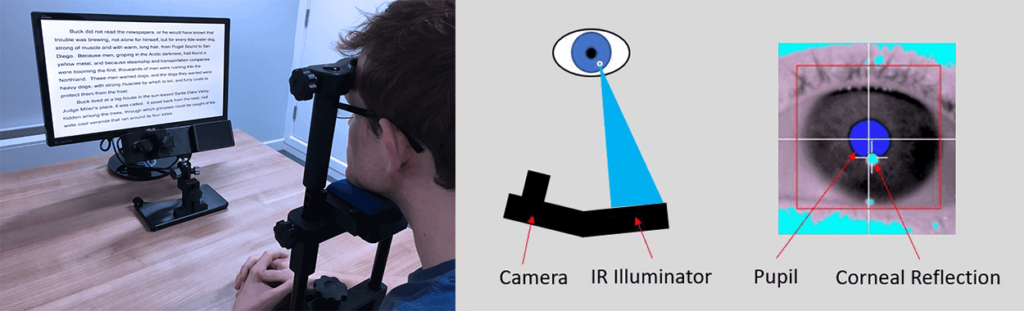
\includegraphics[width=1\textwidth,height=\textheight]{images/SR_research.png}

}

\caption{Image source:
\href{https://www.sr-research.com/about-eye-tracking/}{SR Research} (all
rights reserved)}

\end{figure}

\hypertarget{eye-tracking-during-reading}{%
\section{Eye-tracking during
reading}\label{eye-tracking-during-reading}}

\hypertarget{eye-tracking-reading-measures}{%
\subsection{Eye-tracking reading
measures}\label{eye-tracking-reading-measures}}

\begin{itemize}
\tightlist
\item
  inform theories of language processing via linking hypotheses

  \begin{itemize}
  \tightlist
  \item
    linking visual attention to processing
  \end{itemize}
\item
  typically, we compare reading times as a function of some manipulation
\end{itemize}

e.g., The They key on the cabinets is on the table.

\begin{itemize}
\tightlist
\item
  longer reading times
\end{itemize}

\hypertarget{region-of-interest-roi}{%
\subsection{Region of interest (ROI)}\label{region-of-interest-roi}}

\begin{itemize}
\tightlist
\item
  can be anything on-screen

  \begin{itemize}
  \tightlist
  \item
    sentence-level
  \item
    word/region-level
  \item
    a certain part of the screen
  \end{itemize}
\end{itemize}

\begin{figure}

{\centering \includegraphics[width=1\textwidth,height=\textheight]{images/crit_trial_px03.mov}

}

\end{figure}

\hypertarget{measures-dependent-variables}{%
\subsection{Measures (dependent
variables)}\label{measures-dependent-variables}}

\begin{itemize}
\tightlist
\item
  what we measure = \emph{dependent} variables (usually\ldots)

  \begin{itemize}
  \tightlist
  \item
    their value \emph{depends} on some \emph{predictor} (e.g., word
    frequency)
  \end{itemize}
\end{itemize}

\begin{itemize}
\tightlist
\item
  measures of duration (time spent on a region)

  \begin{itemize}
  \tightlist
  \item
    first fixation
  \item
    first-pass reading time
  \item
    regression path duration
  \item
    total reading time
  \end{itemize}
\item
  data type: \emph{continuous}
\end{itemize}

\begin{itemize}
\tightlist
\item
  measures of revisits

  \begin{itemize}
  \tightlist
  \item
    number of fixations
  \item
    number of regressions in/out
  \item
    regression in/out (yes or no)
  \item
    probability of regressions in/out (0:1)
  \end{itemize}
\item
  data type: binary (0,1) or count
\end{itemize}

\hypertarget{independent-variables}{%
\subsection{Independent variables}\label{independent-variables}}

\begin{itemize}
\tightlist
\item
  what can influence reading measures? (Juhasz and Pollatsek 2011;
  Rayner and Liversedge 2011; Warren 2011; Clifton and Staub 2011)

  \begin{itemize}
  \tightlist
  \item
    some examples:
  \end{itemize}
\end{itemize}

\begin{itemize}
\tightlist
\item
  Word properties

  \begin{itemize}
  \tightlist
  \item
    word frequency
  \item
    word length
  \end{itemize}
\end{itemize}

\begin{itemize}
\tightlist
\item
  Sentence-level influences

  \begin{itemize}
  \tightlist
  \item
    context (i.e., prediction)
  \item
    semantic or grammatical manipulations
  \end{itemize}
\end{itemize}

\begin{itemize}
\tightlist
\item
  Inter- and intra-individual

  \begin{itemize}
  \tightlist
  \item
    domain-specific expertise
  \item
    reading skill level
  \end{itemize}
\end{itemize}

\hypertarget{what-do-these-measures-tell-us}{%
\subsection{What do these measures tell
us?}\label{what-do-these-measures-tell-us}}

\begin{itemize}
\tightlist
\item
  eye-tracking during reading can tell use \emph{when} and \emph{where}
  processing costs are incurred
\item
  \emph{early measures} involve ``first contact with a word'' or region:
  first-fixation, first-pass reading time (Vasishth, von der Malsburg,
  and Engelmann 2013, 126)
\item
  \emph{late measures} involve regressions to a region: e.g., total
  reading time

  \begin{itemize}
  \tightlist
  \item
    may also include `spillover' effects from early processing
  \end{itemize}
\item
  eye-tracking during reading measures can therefore tell us about
  stages of processing
\end{itemize}

\hypertarget{references}{%
\section*{References}\label{references}}

\hypertarget{refs}{}
\begin{CSLReferences}{1}{0}
\leavevmode\vadjust pre{\hypertarget{ref-clifton_syntactic_2011}{}}%
Clifton, Charles, and Adrian Staub. 2011. {``Syntactic Influences on Eye
Movements During Reading.''} In \emph{Oxford Handbook of Eye Movements}.
Oxford University Press.
\url{https://doi.org/10.1093/oxfordhb/9780199539789.013.0049}.

\leavevmode\vadjust pre{\hypertarget{ref-juhasz_lexical_2011}{}}%
Juhasz, Barbara J, and Alexander Pollatsek. 2011. {``Lexical Influences
on Eye Movements in Reading.''} In \emph{Oxford Handbook of Eye
Movements}.

\leavevmode\vadjust pre{\hypertarget{ref-rayner_eye_2009-1}{}}%
Rayner, Keith. 2009. \emph{Eye Movements and Attention in Reading, Scene
Perception, and Visual Search}. Vol. 62.
\url{https://doi.org/10.1080/17470210902816461}.

\leavevmode\vadjust pre{\hypertarget{ref-rayner_linguistic_2011}{}}%
Rayner, Keith, and Simon P Liversedge. 2011. {``Linguistic and Cognitive
Influences on Eye-Movements During Reading.''} In \emph{Oxford Handbook
of Eye Movements}.

\leavevmode\vadjust pre{\hypertarget{ref-vasishth_what_2013}{}}%
Vasishth, Shravan, Titus von der Malsburg, and Felix Engelmann. 2013.
{``What Eye Movements Can Tell Us about Sentence Comprehension.''}
\emph{Wiley Interdisciplinary Reviews: Cognitive Science} 4 (2):
125--34. \url{https://doi.org/10.1002/wcs.1209}.

\leavevmode\vadjust pre{\hypertarget{ref-warren_influence_2011}{}}%
Warren, Tessa. 2011. {``The Influence of Implausibility and Anomaly on
Eye Movements During Reading.''} In \emph{Oxford Handbook of Eye
Movements}.

\end{CSLReferences}



\end{document}
